% GNUPLOT: LaTeX picture with Postscript
\begingroup
  \makeatletter
  \providecommand\color[2][]{%
    \GenericError{(gnuplot) \space\space\space\@spaces}{%
      Package color not loaded in conjunction with
      terminal option `colourtext'%
    }{See the gnuplot documentation for explanation.%
    }{Either use 'blacktext' in gnuplot or load the package
      color.sty in LaTeX.}%
    \renewcommand\color[2][]{}%
  }%
  \providecommand\includegraphics[2][]{%
    \GenericError{(gnuplot) \space\space\space\@spaces}{%
      Package graphicx or graphics not loaded%
    }{See the gnuplot documentation for explanation.%
    }{The gnuplot epslatex terminal needs graphicx.sty or graphics.sty.}%
    \renewcommand\includegraphics[2][]{}%
  }%
  \providecommand\rotatebox[2]{#2}%
  \@ifundefined{ifGPcolor}{%
    \newif\ifGPcolor
    \GPcolorfalse
  }{}%
  \@ifundefined{ifGPblacktext}{%
    \newif\ifGPblacktext
    \GPblacktexttrue
  }{}%
  % define a \g@addto@macro without @ in the name:
  \let\gplgaddtomacro\g@addto@macro
  % define empty templates for all commands taking text:
  \gdef\gplbacktext{}%
  \gdef\gplfronttext{}%
  \makeatother
  \ifGPblacktext
    % no textcolor at all
    \def\colorrgb#1{}%
    \def\colorgray#1{}%
  \else
    % gray or color?
    \ifGPcolor
      \def\colorrgb#1{\color[rgb]{#1}}%
      \def\colorgray#1{\color[gray]{#1}}%
      \expandafter\def\csname LTw\endcsname{\color{white}}%
      \expandafter\def\csname LTb\endcsname{\color{black}}%
      \expandafter\def\csname LTa\endcsname{\color{black}}%
      \expandafter\def\csname LT0\endcsname{\color[rgb]{1,0,0}}%
      \expandafter\def\csname LT1\endcsname{\color[rgb]{0,1,0}}%
      \expandafter\def\csname LT2\endcsname{\color[rgb]{0,0,1}}%
      \expandafter\def\csname LT3\endcsname{\color[rgb]{1,0,1}}%
      \expandafter\def\csname LT4\endcsname{\color[rgb]{0,1,1}}%
      \expandafter\def\csname LT5\endcsname{\color[rgb]{1,1,0}}%
      \expandafter\def\csname LT6\endcsname{\color[rgb]{0,0,0}}%
      \expandafter\def\csname LT7\endcsname{\color[rgb]{1,0.3,0}}%
      \expandafter\def\csname LT8\endcsname{\color[rgb]{0.5,0.5,0.5}}%
    \else
      % gray
      \def\colorrgb#1{\color{black}}%
      \def\colorgray#1{\color[gray]{#1}}%
      \expandafter\def\csname LTw\endcsname{\color{white}}%
      \expandafter\def\csname LTb\endcsname{\color{black}}%
      \expandafter\def\csname LTa\endcsname{\color{black}}%
      \expandafter\def\csname LT0\endcsname{\color{black}}%
      \expandafter\def\csname LT1\endcsname{\color{black}}%
      \expandafter\def\csname LT2\endcsname{\color{black}}%
      \expandafter\def\csname LT3\endcsname{\color{black}}%
      \expandafter\def\csname LT4\endcsname{\color{black}}%
      \expandafter\def\csname LT5\endcsname{\color{black}}%
      \expandafter\def\csname LT6\endcsname{\color{black}}%
      \expandafter\def\csname LT7\endcsname{\color{black}}%
      \expandafter\def\csname LT8\endcsname{\color{black}}%
    \fi
  \fi
    \setlength{\unitlength}{0.0500bp}%
    \ifx\gptboxheight\undefined%
      \newlength{\gptboxheight}%
      \newlength{\gptboxwidth}%
      \newsavebox{\gptboxtext}%
    \fi%
    \setlength{\fboxrule}{0.5pt}%
    \setlength{\fboxsep}{1pt}%
    \definecolor{tbcol}{rgb}{1,1,1}%
\begin{picture}(9936.00,3600.00)%
    \gplgaddtomacro\gplbacktext{%
      \csname LTb\endcsname%%
      \put(858,440){\makebox(0,0)[r]{\strut{}$0$}}%
      \put(858,1028){\makebox(0,0)[r]{\strut{}$2000$}}%
      \put(858,1616){\makebox(0,0)[r]{\strut{}$4000$}}%
      \put(858,2203){\makebox(0,0)[r]{\strut{}$6000$}}%
      \put(858,2791){\makebox(0,0)[r]{\strut{}$8000$}}%
      \put(858,3379){\makebox(0,0)[r]{\strut{}$10000$}}%
      \put(990,220){\makebox(0,0){\strut{}$515$}}%
      \put(1367,220){\makebox(0,0){\strut{}$525$}}%
      \put(1743,220){\makebox(0,0){\strut{}$535$}}%
      \put(2120,220){\makebox(0,0){\strut{}$545$}}%
      \put(2496,220){\makebox(0,0){\strut{}$555$}}%
      \put(2873,220){\makebox(0,0){\strut{}$565$}}%
      \put(3250,220){\makebox(0,0){\strut{}$575$}}%
      \put(3626,220){\makebox(0,0){\strut{}$585$}}%
      \put(4003,220){\makebox(0,0){\strut{}$595$}}%
      \put(4379,220){\makebox(0,0){\strut{}$605$}}%
      \put(4756,220){\makebox(0,0){\strut{}$615$}}%
      \put(5133,220){\makebox(0,0){\strut{}$625$}}%
      \put(5509,220){\makebox(0,0){\strut{}$635$}}%
      \put(5886,220){\makebox(0,0){\strut{}$645$}}%
      \put(6263,220){\makebox(0,0){\strut{}$655$}}%
      \put(6639,220){\makebox(0,0){\strut{}$665$}}%
      \put(7016,220){\makebox(0,0){\strut{}$675$}}%
      \put(7392,220){\makebox(0,0){\strut{}$685$}}%
      \put(7769,220){\makebox(0,0){\strut{}$695$}}%
      \put(8146,220){\makebox(0,0){\strut{}$705$}}%
      \put(8522,220){\makebox(0,0){\strut{}$715$}}%
      \put(8899,220){\makebox(0,0){\strut{}$725$}}%
      \put(9275,220){\makebox(0,0){\strut{}$735$}}%
    }%
    \gplgaddtomacro\gplfronttext{%
      \csname LTb\endcsname%%
      \put(99,1909){\rotatebox{-270}{\makebox(0,0){\strut{}}}}%
      \put(5264,-66){\makebox(0,0){\strut{}}}%
      \csname LTb\endcsname%%
      \put(3213,3181){\makebox(0,0)[r]{\strut{} spektrální čáry Neonu}}%
      \csname LTb\endcsname%%
      \put(3213,2961){\makebox(0,0)[r]{\strut{} spektrální čáry Helia}}%
    }%
    \gplbacktext
    \put(0,0){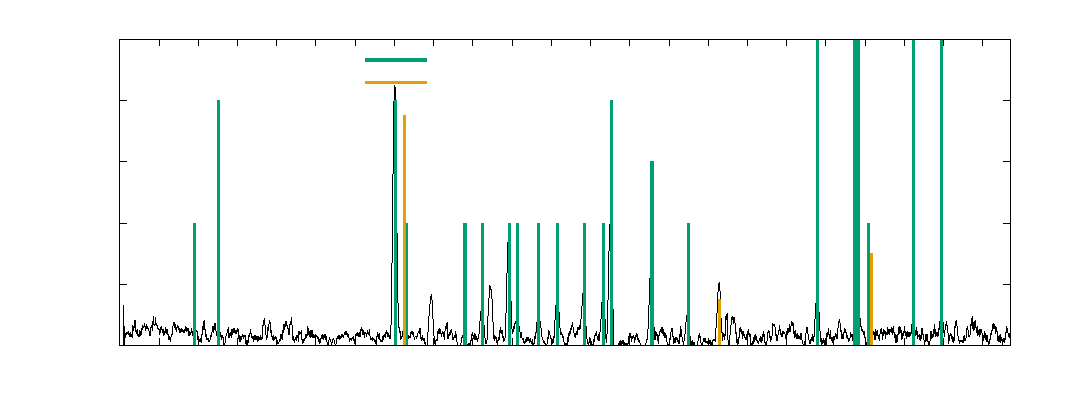
\includegraphics[width={496.80bp},height={180.00bp}]{spektrum}}%
    \gplfronttext
  \end{picture}%
\endgroup
